\section{File System}
L' organizzazione di un file system dipende strettamente da quale sistema operativo si sta utilizzando e da che tipo di file system si è deciso di utilizzare.
Più in generale analizzeremo un file system basato su file e directory su partizioni del disco fisico.

Costruiremo questa astrazione su un disco virtuale cioè vedendo il disco come un array di blocchi.

In generale un file system è la parte del sistema operativo che fornisce i meccanismi necessari per l' accesso e l' archiviazione delle informazioni in memoria secondaria.
Ci permette di costruire le astrazioni:
\begin{itemize}
    \item \emph{file}: unità logica di memorizzazione
    \item \emph{directory}: insieme di file e di altre directory
    \item \emph{partizione}: insieme di file associato ad un particolare dipositivo fisico o una porzione di esso
\end{itemize}

\subsection{Astrazioni utili}
\subsubsection{File}
Un file porta con se, oltre al contenuto, tante altre informazioni come ad esempio:
\begin{itemize}
    \item nome: ogni file ha un nome che lo identifica internamente ad una directory
    \item tipo: indica l' appartenza ad una classe (eseguibile, batch, testo, ecc)

    \item estensione: in alcuni file system è evidenziato espressamente da una stringa divisa da un punto.
    In alcuni sistemi operativi è usato per interpretare il contenuto del file stesso e scegliere con quale applicazione aprirlo ed utilizzarlo
    
    \item dimensione: espressa in byte o in blocchi (o record logici)

    \item proprietario del file e permessi
    \item gruppo proprietario del file e permessi
    \item permessi sul file degli altri utenti
    
    \item indirizzo puntatore alla memoria secondaria
    \item data ed ora di creazione e di ultima modifica
\end{itemize}

\subsubsection{Directory}
Una directory contiene un insieme di file ed altre directory ed è a sua volta contenuta in altre directory.
Tramite questo meccanismo possiamo costruire una gerarchia del file system con alla radice un qualcosa che dipende strettamente dal sistema operativo, in linux/UNIX abbiamo la directory root \verb{\{, su windows il nome del disco \verb{C://{.

Con le directory arriva il concetto di pathname di un file, è il percorso di directory che portano dalla radice al singolo file, la pathname ci permette di creare file con lo stesso nome nello stesso file system a patto che non condividano la stessa pathname (e quindi la stessa directory).

\subsubsection{Partizione}
Una partizione è una porzione di un disco fisico usata per inserire un determinato file system.
Sono cioè dei dischi logici mappati sullo stesso disco.

In UNIX abbiamo almeno due partizioni obbligatorie: la partizione di swap e la partizione del file system che contiene i file dell' utente.

Volendo possiamo anche costruire una astrazione di file system su una rete: un network file system che si sviluppa attraverso diversi dispositivi nella rete.

\subsection{Organizzazione del file system}
\begin{figure}[H]
    \centering
    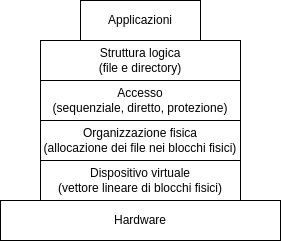
\includegraphics[width=200px]{images/11_File_System/file_system_structure.png}
\end{figure}
\begin{itemize}
    \item il dispositivo virtuale è l' interfaccia che usa il file system per interfacciarsi con il disco vero e proprio, dal suo punto di vista il disco è un vettore lineare di blocchi fisici, quindi ci si riferisce tramite un indice numerico.

    \item l' organizzazione fisica si occupa di allocare i file e le directory, e le relative informazioni, sui blocchi fisici cioè nelle celle dell' array virtuale che stiamo immaginando.
    Di base gestiscono l' accesso a questo array.

    \item il livello di accesso si occupa di permettere l' accesso controllato al file system, leggere i file in maniera sequenziale, muoversi e modificarlo; inoltre implementa i meccanismi di protezione dei file tramite la matrice dei permessi.
    In questo livello un file è visto come un insieme di record e l' accesso a questo elenco è gestito dal sistema operativo su richiesta della applicazione.

    \item la struttura logica implementa il file system tree navigabile e modificabile dagli utenti.
\end{itemize}

In base all' organizzazione che decidiamo di costruire possiamo avere:
\begin{itemize}
    \item organizzazione ad albero: si parte da una directory radice, ogni directory può contenere altre directory ed ogni directory può contenere file a piacere
    
    \item organizzazione a grafo diretto aciclico: si tratta di una organizzazione ad albero che permette l' utilizzo dei link, cioè di alias per i file all' interno del file system, ma in altri pathname
\end{itemize}

\subsection{Gestione del file system}
Per gestire il file system dobbiamo chiamare il sistema operativo che ci mette a disposizione alcune utility per:
\begin{itemize}
    \item creare e cancellare directory
    \item aggiungere e cancellare file
    \item listare il contenuto delle directory
    \item attraversare le directory
\end{itemize}

\subsection{Accesso al file system}
\subsubsection{Rappresentazione del file}
Per rappresentare i file si usano delle strutture dati dette \emph{descrittore di file}: questa struttura memorizza gli attributi necessari e devono essere mantenuti in memoria secondaria in quanto persistenti.
In UNIX il descrittore di file è detto \emph{i-node}.

\subsubsection{Rappresentazione della directory}
Dato che ogni file appartiene ad una directory, ogni directory deve mantenere dei collegamenti ai file che contiene.
Un modo per fare ciò è rappresentare la directory in una forma tabellare il cui contenuto sono proprio i descrittori dei file.

Un secondo modo per fare ciò è costruire una singola tabella per i descrittori dei file (\emph{i-list}) e nella tabella associata alla directory inserire i puntatori agli elementi di questa lista.
In questo modo concentro i descrittori dei file tutti in un punto ma aumento l' overhead per l' accesso ai file dovendo passare per questo puntatore.

\subsubsection{Accesso ai file}
E' compito del sistema operativo permettere l' accesso ai file mediante operazioni di accesso:
\begin{itemize}
    \item in lettura: si legge l' array di record logici associati al file (in UNIX un record logico ha dimensione 1 byte)
    \item in scrittura: si inseriscono nuovi record logici all' interno del file
\end{itemize}
Ogni operazione richiede la localizzazione di varie informazioni che si trovano su disco, come ad esempio: gli indirizzi dei record dei file, gli attributi del file ed i record logici stessi, tuttavia fare accessi al disco è sempre oneroso!

Per migliorare l' efficienza il sistema operativo mantiene in memoria una struttura che registra i file \emph{aperti}, si mantengono in particolare il puntatore al file e la posizione sul disco oltre che altre informazioni per i controlli veloci, inoltre i file aperti vengono copiati interamente o in parte nella memoria centrale in modo da avere un accesso più veloce: \emph{memory mapping}.

Per interagire con i file occorrono quindi due operazioni obbligatorie:
\begin{itemize}
    \item apertura del file: si inserisce una nuova entrata nella tabella dei file aperti ed eventualmente si mappa in memoria centrale il contenuto del file
    \item chiusura del file: si salva il file in memoria secondaria e si elimina l' elemento dalla tabella dei file aperti, si fa in pratica il cleanup della apertura
\end{itemize}

\subsubsection{Metodi di accesso ai file}
Possiamo accedere al file con varie modalità:
\begin{itemize}
    \item accesso sequenziale: si parte dal primo blocco logico e si va in sequenza, quindi dobbiamo scorrere tutti i record prima dell' $i$-esimo per accedere al record $i$.
    Abbiamo le operazioni:
    \begin{verbatim}
    readnext(f, &V)
        // lettura del prossimo record logico
    writenext(f, V)
        // scrittura del prossimo record logico
    \end{verbatim}
    Ogni accesso sposta in avanti il cursore del file.

    \item accesso diretto: il file è visto come un array di record logici, ci si può accedere direttamente indicizzandolo:
    \begin{verbatim}
    readd(f, i, &V)
        // legge il record i-esimo del file f
    writed(f, i, V)
        // scrive sul record i-esimo del file f
    \end{verbatim}
    In questo modo non devo perdere tempo nella lettura dei record antecedenti se voglio fare un accesso nel mezzo.

    \item accesso a indice: ad ogni file si associa un' altra struttura che contiene l' indice delle informazioni contenute nel file.
    Facciamo quindi l' accesso a questa struttura mediante una chiave e dalla struttura otteniamo l' indice di quella chiave per accedere al file:
    \begin{verbatim}
        readk(f, key, &V)
            // accediamo all' indice associato alla chiave
        writek(f, key, V)
            // scrivimo sul record associato alla chiave
    \end{verbatim}
    Si tratta di fatto di un indirizzamento indiretto:
    \begin{figure}[H]
        \centering
        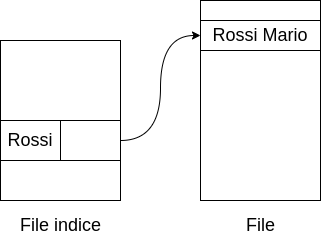
\includegraphics[width=200px]{images/11_File_System/accesso_a_indice.png}
    \end{figure}
    Questo tipo di accesso è principalmente usato per file molto grandi, in questi casi in memoria centrale si inserisce il file indice e poi a necessità si legge il file reale o una sua porzione.

\end{itemize}
Questi metodi di accesso sono indipendenti dal dispositivo e dalla tecnica di allocazione dei blocchi in memoria secondaria in quanto per il programmatore un file è un array di blocchi logici contigui.

\subsection{Organizzazione fisica del file system}
Ogni dispositivo di memorizzazione secondaria viene partizionato in blocchi (record fisici) quindi i trasferimenti tramite lo spazio di I/O da/verso i dispositivi avvengono per blocchi di dimensione costante che coincidono con il settore del disco.
Dal punto di vista dei processi invece l'unità di trasferimento è il record logico.

Di solito la dimensione del blocco è di molto maggiore rispetto alla dimensione del record logico quindi può contenerne molti di più.
E' compito del sistema operativo mappare i record logici all' interno dei blocchi e quindi dei settori fisici.

\subsubsection{Allocazione contigua}
Possiamo mappare ogni file su blocchi fisicamente contigui, in questo modo la ricerca è semplice perché una volta trovato il primo blocco dobbiamo solo leggere, inoltre abbiamo un accesso sequenziale e diretto.

Tuttavia in questa maniera abbiamo una frammentazione esterna perché man mano che si riempie il disco rimangono zone contigue sempre più piccole spesso inutilizzabili, è necessario eseguire una compattazione in questi casi.
Aumenta altresì il costo della ricerca dello spazio libero per l' allocazione di un nuovo file e non è sempre permesso accrescere le dimensioni dei file perché una volta raggiunto un certo limite lo spazio contiguo finisce.
\begin{figure}[H]
    \centering
    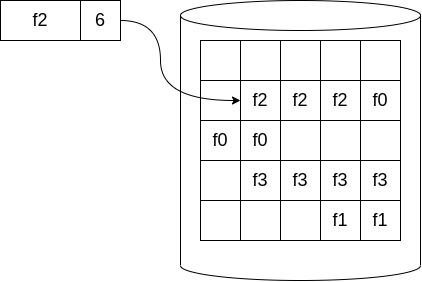
\includegraphics[width=200px]{images/11_File_System/allocazione_contigua.png}
\end{figure}

\subsubsection{Allocazione a lista concatenata}
I blocchi sui quali viene mappato ogni file sono organizzati in una lista concatenata.
Con questa tecnica se mi servono $k$ blocchi mi basterà avere $k$ blocchi liberi in qualsiasi disposizione, non per forza contigui.

Con questa tecnica non c'è frammentazione esterna, c'è un minor costo nella ricerca dei blocchi ed ho un veloce accesso sequenziale.

D' altro canto se il link tra alcuni blocchi viene danneggiato ho perso la struttura da quel punto in poi, in ogni blocco poi devo tenere un po' di spazio per mantenere il puntatore al blocco successivo.
Inoltre non è permesso l' accesso diretto in quanto devo sempre seguire tutta la catena e la ricerca di un blocco è lenta.
\begin{figure}[H]
    \centering
    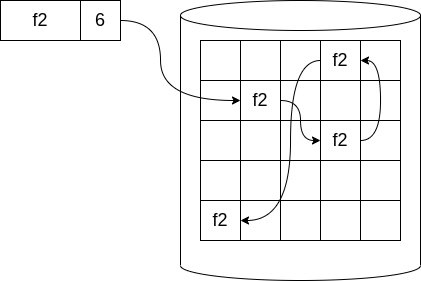
\includegraphics[width=200px]{images/11_File_System/allocazione_lista_concatenata.png}
\end{figure}

\subsubsection{Allocazione a lista doppiamente concatenata}
Una variazione dell' allocazione precedente che prevede che ogni blocco ponga 2 puntatori, uno per andare al prossimo blocco ed uno per andare al precedente.
In questo modo aumenta la robustezza del file system in quanto se un blocco mi si corrompe posso comunque riuscire a ritrovare i blocchi successivi.

\begin{figure}[H]
    \centering
    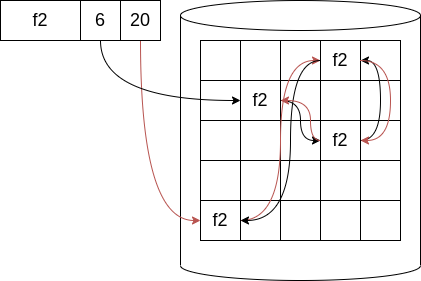
\includegraphics[width=200px]{images/11_File_System/allocazione_lista_doppiamente_concatenata.png}
\end{figure}

\subsubsection{File Allocation Table}
Si usano alcuni blocchi per mantenere un elenco dei puntatori dei blocchi.
Questo elenco può essere copiato in memoria centrale per ottimizzare l' accesso diretto.

\subsubsection{Allocazione ad indice}
Ad ogni file associamo un indice costruito su un blocco in cui sono contenuti tutti gli indirizzi dei blocchi su cui è allocato il file.
Con questo metodo ci basta leggere un singolo blocco per avere l' elenco dei blocchi che ospitano un file, abbiamo pertanto la possibilità di un accesso diretto ed anche una maggiore velocità di accesso.

Tuttavia è una soluzione che non scala in quanto un singolo blocco può tenere in memoria fino ad un certo numero di indirizzi di blocco quindi se il file diventa troppo grande non potrò più usare un solo blocco come indice.

Il file system deve quindi tenere in memoria l' associazione tra il file ed il blocco indice ed all' occasione cashare il blocco indice per velocizzare gli accessi.


